\documentclass{article}

% Importing packages
\usepackage{amsmath, amsthm, amssymb, amsfonts}
\usepackage{thmtools}
\usepackage{graphicx}
\usepackage{setspace}
\usepackage{float}
\usepackage[colorlinks=true, linkcolor=Blue]{hyperref}
\usepackage[utf8]{inputenc}
\usepackage{framed}
\usepackage[dvipsnames]{xcolor}
\usepackage{tcolorbox}
\newtcolorbox{mymathbox}[1][]{colback=white, sharp corners, #1}

\title{Complex Potential and Complex Velocity}
\author{Mauro Patimo}
\begin{document}
\maketitle

Since the potential and the streamline have a very specific relation
\begin{equation}
    u=\frac{d\phi}{dx}=\frac{d\psi}{dy}, \quad v=\frac{d\phi}{dy}=-\frac{d\psi}{dx}
\end{equation}
These two equations fullfill the Cauchy-Riemann conditions, so we can write the potential as a complex function:
\begin{equation}
    F(z)=\phi(x,y)+i\psi(x,y)
\end{equation}
where $z=x+iy$, and $i=\sqrt{-1}$.\\
This complex analytical function is called \textbf{complex potential}, and it allows us to describe the behaviour of two independent variables into a single complex variable.\\
\begin{equation}
    \frac{dF}{dz}=\frac{dF}{dx}=\frac{1}{i}\frac{dF}{dy}=\frac{d\phi}{dx}+i\frac{d\psi}{dx}=-i\frac{d\phi}{dy}+\frac{d\psi}{dy}
\end{equation}
We can then write the complex potential as:
\begin{equation}
    \frac{dF}{dz}=u-iv=\bar{\omega}
\end{equation}
Where $\bar{\omega}$ is the complex conjugate of $\omega=u+iv$.\\
Complex quantities can be expressed as x and y components in the complez plane (Argand diagram):
\begin{figure}
    \centering
    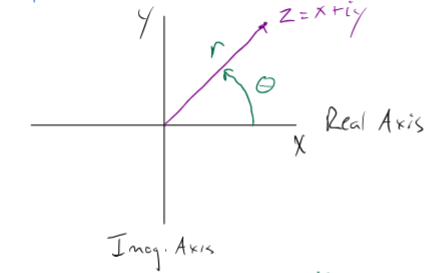
\includegraphics[width=0.5\textwidth]{Argand Diagram.png}
    \caption{Argand Diagram}
    \label{fig:Argand Diagram}
\end{figure}
Remember Euler's formula:
\begin{align*}
    e^{i\theta}&=\cos\theta+i\sin\theta \\
    z &= x+iy = r(\cos\theta+i\sin\theta)=re^{i\theta}
\end{align*}
For example:
\begin{align*}
    \frac{1}{z}&=\frac{1}{x+iy}\frac{x-iy}{x^2+y^2}=\frac{x}{x^2+y^2}-i\frac{y}{x^2+y^2} \\
    \frac{1}{z}&=z^{-1}=\frac{1}{r}e^{-i\theta}=\frac{1}{r}(\cos\theta-i\sin\theta)=\underbrace{\frac{rcos\theta}{r^2}}_{\frac{x}{x^2+y^2}}-\underbrace{i\frac{rsin\theta}{r^2}}_{\frac{y}{x^2+y^2}}\\
\end{align*}
So a basic Potential Flow solution in complex form looks like:
\begin{equation}
    F(z)=\underbrace{U_\infty(xcos\alpha+ysin\alpha)}_\phi+i\underbrace{U_\infty(ycos\alpha-xsin\alpha)}_\psi
\end{equation}
\begin{align*}
    F(z)&=U_\infty e^{i\alpha}z \\
    \bar{\omega}&=\frac{dF}{dz}=U_\infty e^{i\alpha}=U_\infty cos\alpha-iU_\infty sin\alpha=u-iv\\
\end{align*}
A source/sink in complex form is:
\begin{equation}
    F(z)=\frac{\sigma}{2\pi}lnr+i\frac{\sigma}{2\pi}\theta=\frac{\sigma}{2\pi}\ln z
\end{equation}
and
\begin{align*}
    \frac{dF}{dz}=\frac{\sigma}{2\pi z}=\frac{\sigma}{2\pi r}[cos\theta-i\sin\theta]
\end{align*}
For a vortex:
\begin{equation}
    F(z)=\frac{\Gamma}{2\pi}lnz=\frac{\Gamma}{2\pi}lnr-i\frac{\Gamma}{2\pi}\theta
\end{equation}
and
\begin{align*}
    \frac{dF}{dz}=\frac{\Gamma}{2\pi iz}=-\frac{\Gamma}{2\pi r}[sin\theta+i\cos\theta]
\end{align*}
So, a doublet in complex form is:
\begin{align}
    F(z)&=\frac{\mu}{2\pi z}=\frac{\mu}{2\pi r}[cos\theta-i\sin\theta] \\
    \frac{dF}{dz}&=-\frac{\mu}{2\pi z^2}=-\frac{\mu}{2\pi r^2}[cos2\theta-isin2\theta]
\end{align}
We can use $e^{i\theta}$ to rotate the velocity fields. Since $e^{i\theta}$ (where $\theta$ is the angle of rotation) has a unit magnitude, this won't change the mangitude of the function we are multiplying it by.\\
For example, if we want to rotate a doublet by $\theta$:
\begin{align*}
    F(z)&=\frac{\mu}{2\pi z}=\frac{\mu}{2\pi r}[cos\theta-i\sin\theta] \\
    F(z)e^{i\theta}&=\frac{\mu}{2\pi r}[cos\theta-i\sin\theta][cos\theta+i\sin\theta]=\frac{\mu}{2\pi r} \\
    \frac{dF}{dz}e^{i\theta}&=-\frac{\mu}{2\pi r^2}[cos2\theta-isin2\theta][cos\theta+i\sin\theta]=-\frac{\mu}{2\pi r^2}e^{2i\theta}
\end{align*}
If we want to rotate the free stream by $90^\circ$, $\theta=90^\circ$. Thus, $e^{-i\frac{\pi}{2}}=\frac{i}{2}$, which allows the vortex to be orthogonal to the source/sink.\\
\textbf{I higly suggest using this website to understand complex potentials and velocity with intercative exmaples: \href{https://complex-analysis.com/content/mappings.html}{Complex Analysis}}
\end{document}
